\chapter{Surface Facility}
\label{ch:fscf-surf-facil}

%%%%%%%%%%%%%%%%%%%%%%%%%%%%%%%%%%%%%%%%%%%%%%%%%%%%%%%%%%%%%%%%%%%
\section{Existing Surface Facility}
\label{sec:fscf-surf-facil-existing}


The SURF property of 186 acres %consists of 
includes steep terrain and man-made cuts dating from its mining history. %There are approximately 50 buildings and associated site infrastructure in various states of repair. 
There are approximately 50 buildings and associated site infrastructure on the surface to support the main access to underground area from either the Yates Complex or the Ross Complex; the latter will be the main LBNF access. 
A select few of these buildings at the Ross Complex will be upgraded and rehabilitated as necessary for use by LBNF, as will the main utilities. A layout of the overall SURF architectural site plan for the LBNF Project is found in Figure~\ref{fig:archit-site-plan}.
\begin{cdrfigure}[Architectural site plan]{archit-site-plan}{Architectural site plan (HDR) \fixme{add north pointing arrow}\fixme{image fuzzy; orig available?}}
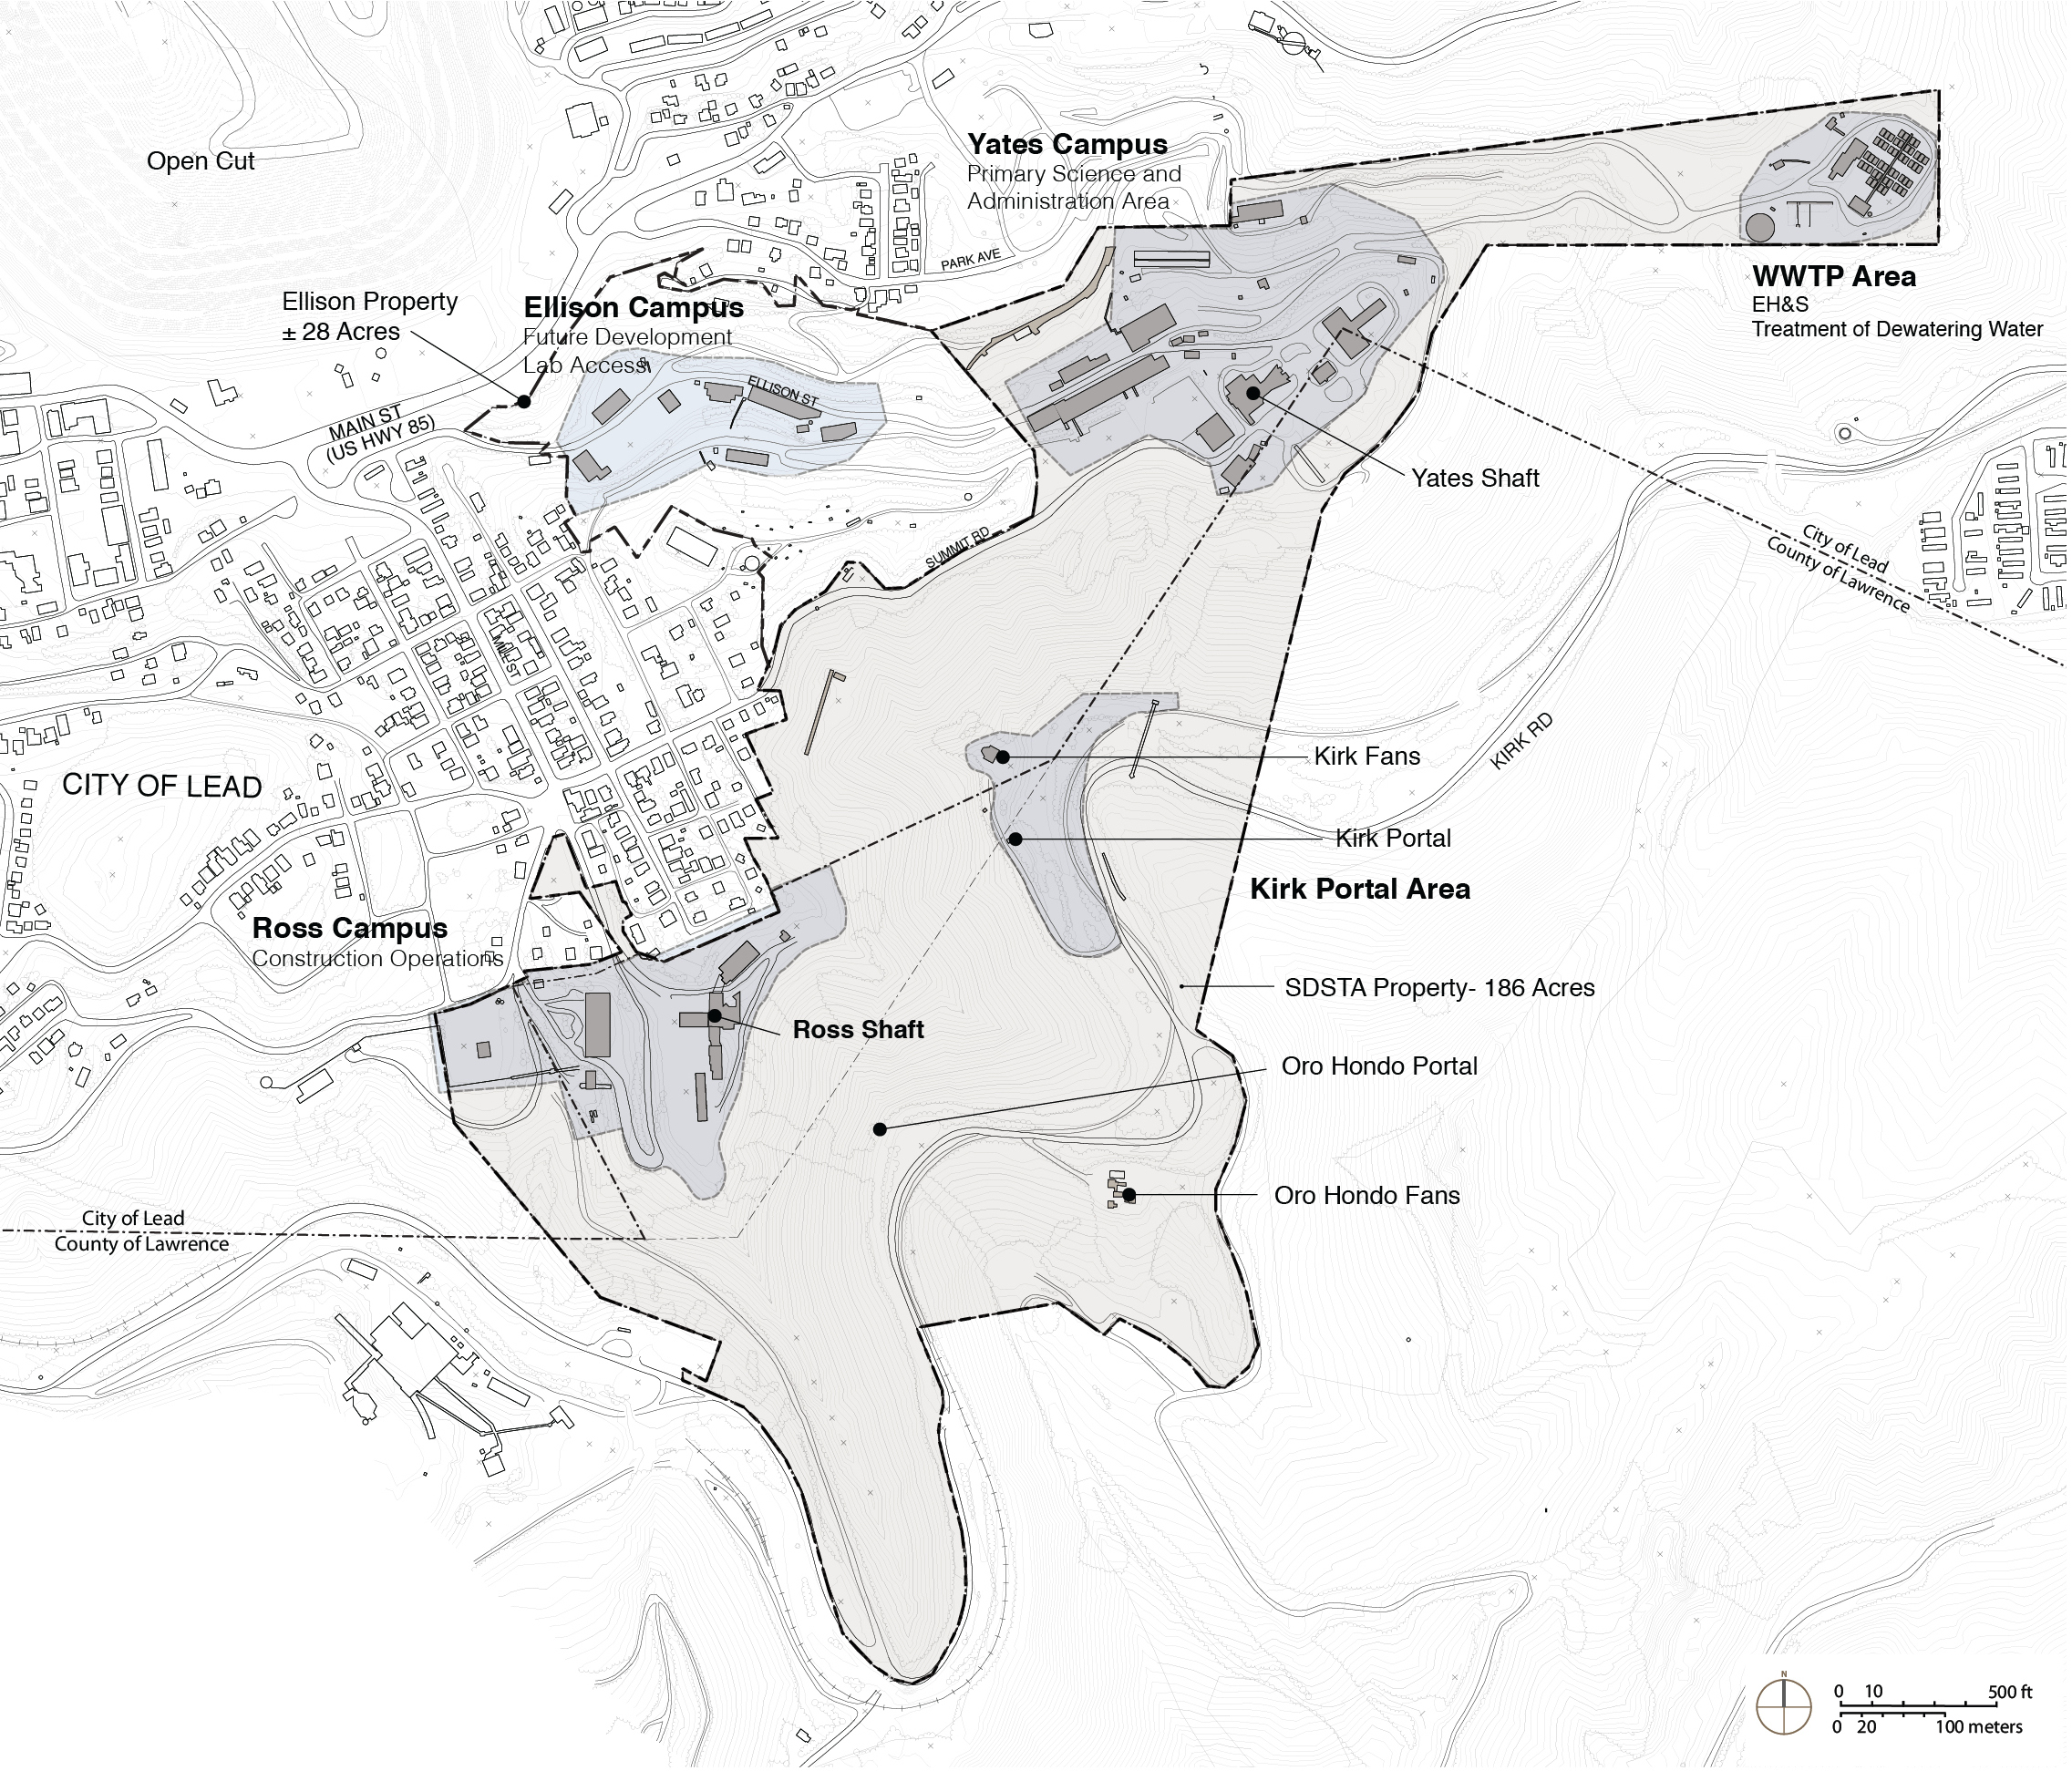
\includegraphics[width=0.8\textwidth]{archit-site-plan}
\end{cdrfigure}
The Ross Complex will house the facility construction operations, the Command and Control Center for the experiment and facility and a new Cryogenics Compressor building, and will continue to house the SURF maintenance and operations functions. Layout of the surface facilities in the vicinity of the Ross Shaft is shown in Figure~\ref{fig:ross-archit-site-plan}.

\begin{cdrfigure}[Ross Complex architectural site plan]{ross-archit-site-plan}{Ross Complex architectural site plan (Arup)}
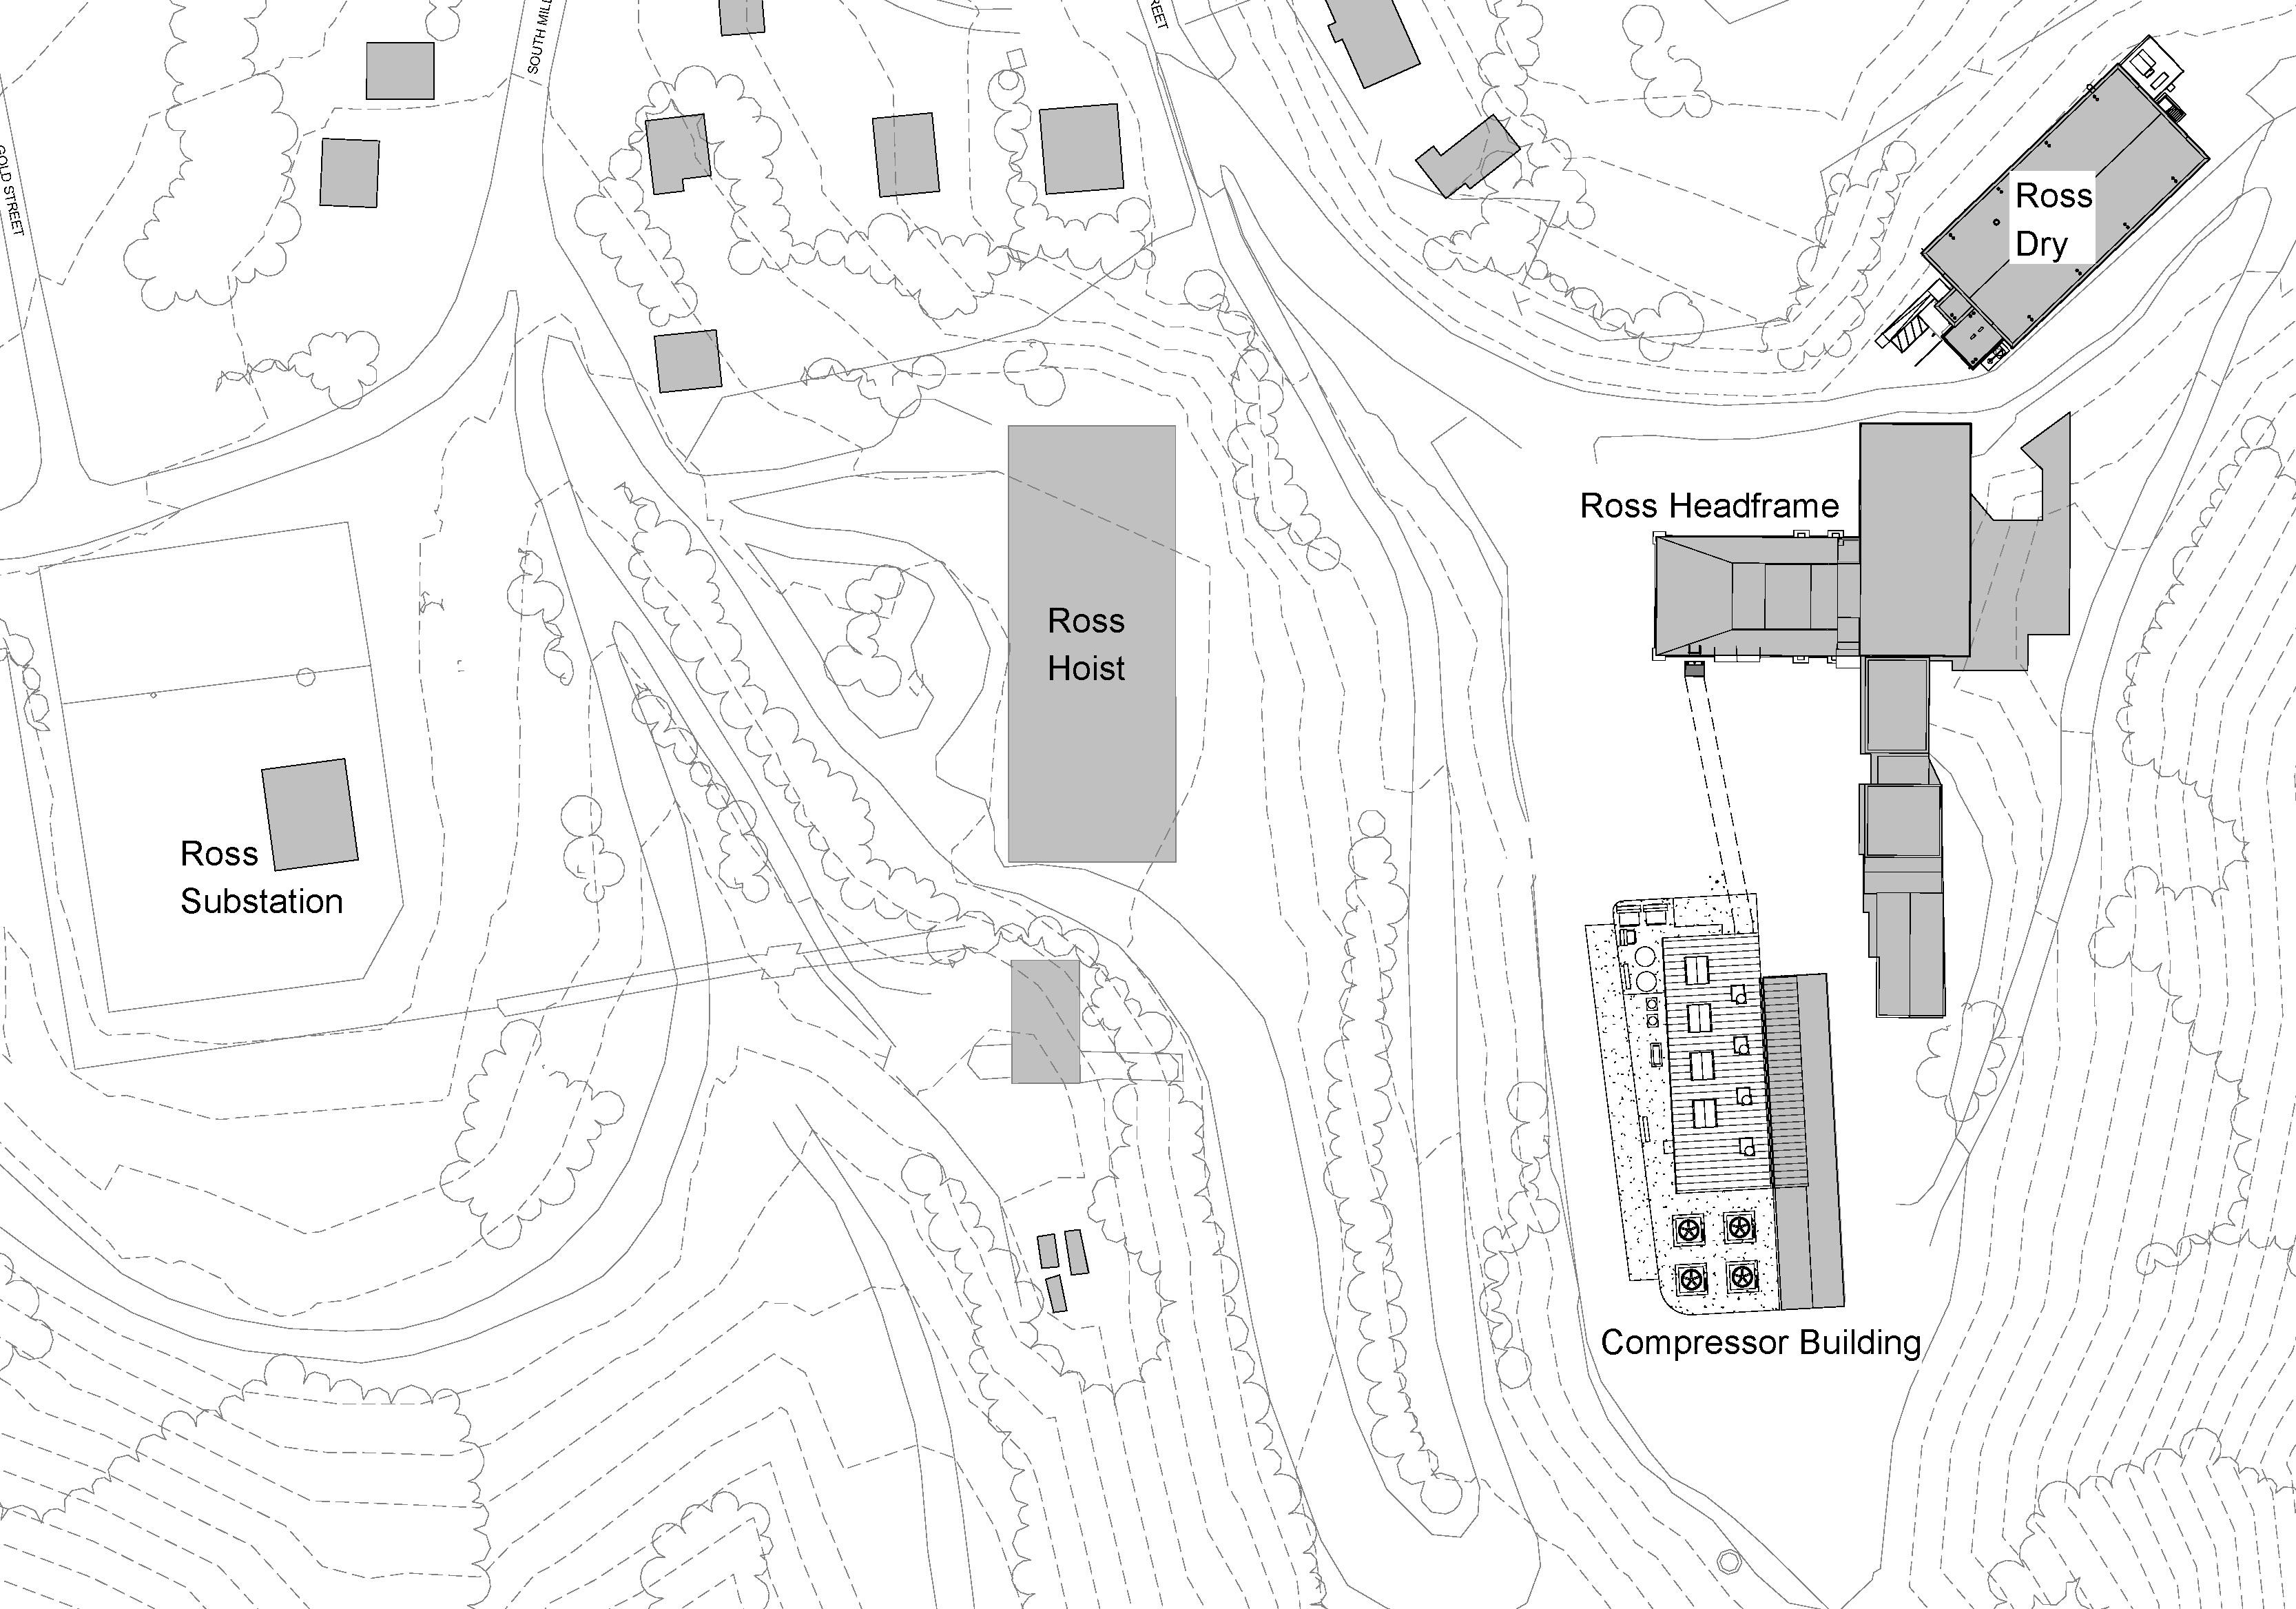
\includegraphics[width=\textwidth]{ross-archit-site-plan}
\end{cdrfigure}

%%%%%%%%%%%%%%%%%%%%%%%%%%%%%%%%%%%%%%%%%%%%%%%%%%%%%%%%%%%%%%%%%%%
\section{Surface Buildings}
\label{sec:fscf-surf-facil-surface-bldg}

Surface buildings for LBNF, existing and planned, include those necessary for safe access and egress to the underground through the Ross Shaft and for office space. The existing buildings will be rehabilitated to comply to codes and to the experiment's requirements. 
%The only new building will provide space for the compressors used to transfer cryogens from new receiving tanks on the surface to the detectors underground. 
The Ross Dry building will be modified to provide space for a surface control room (the Command and Control Center) and offices. The description in this section is excerpted from the 100\% Preliminary Design Report~\cite{arup-100-2011-3a} provided by Arup, USA.

A new building and surrounding concrete slabs are planned in order to provide space for the equipment required for %to allow 
conversion of liquid argon and liquid nitrogen to gaseous form and compression of the nitrogen gas for delivery through the shaft to the underground. % where they are returned to liquid form as described \fixme{find where}. 
The location of this building was selected based on proximity to the shaft and  accessibility for trucks, as thousands of truckloads of argon will be required to fill the detectors underground.

In addition to housing nitrogen compressors inside the building, concrete slabs %are provided 
will be placed around the building %to allow 
for installation of argon and nitrogen receiving dewars (into which the trucks will unload), vaporizers to boil the liquids into gas, an electrical transformer to supply power to the four 1,500-Hp compressors, a standby generator, and cooling towers to reject heat generated through compression. All equipment except the cooling towers and associated circulation pumps is provided by the LBNF Cryogenics Infrastructure~\cite{cryo-design-rpt}. The architectural layout of this building and surrounding equipment is provided in Figure~\ref{fig:compressor-bldg}. 

\begin{cdrfigure}[Architectural layout of LBNF Cryogenics Compressor Building]{compressor-bldg}{Architectural layout of LBNF Cryogenics Compressor Building}
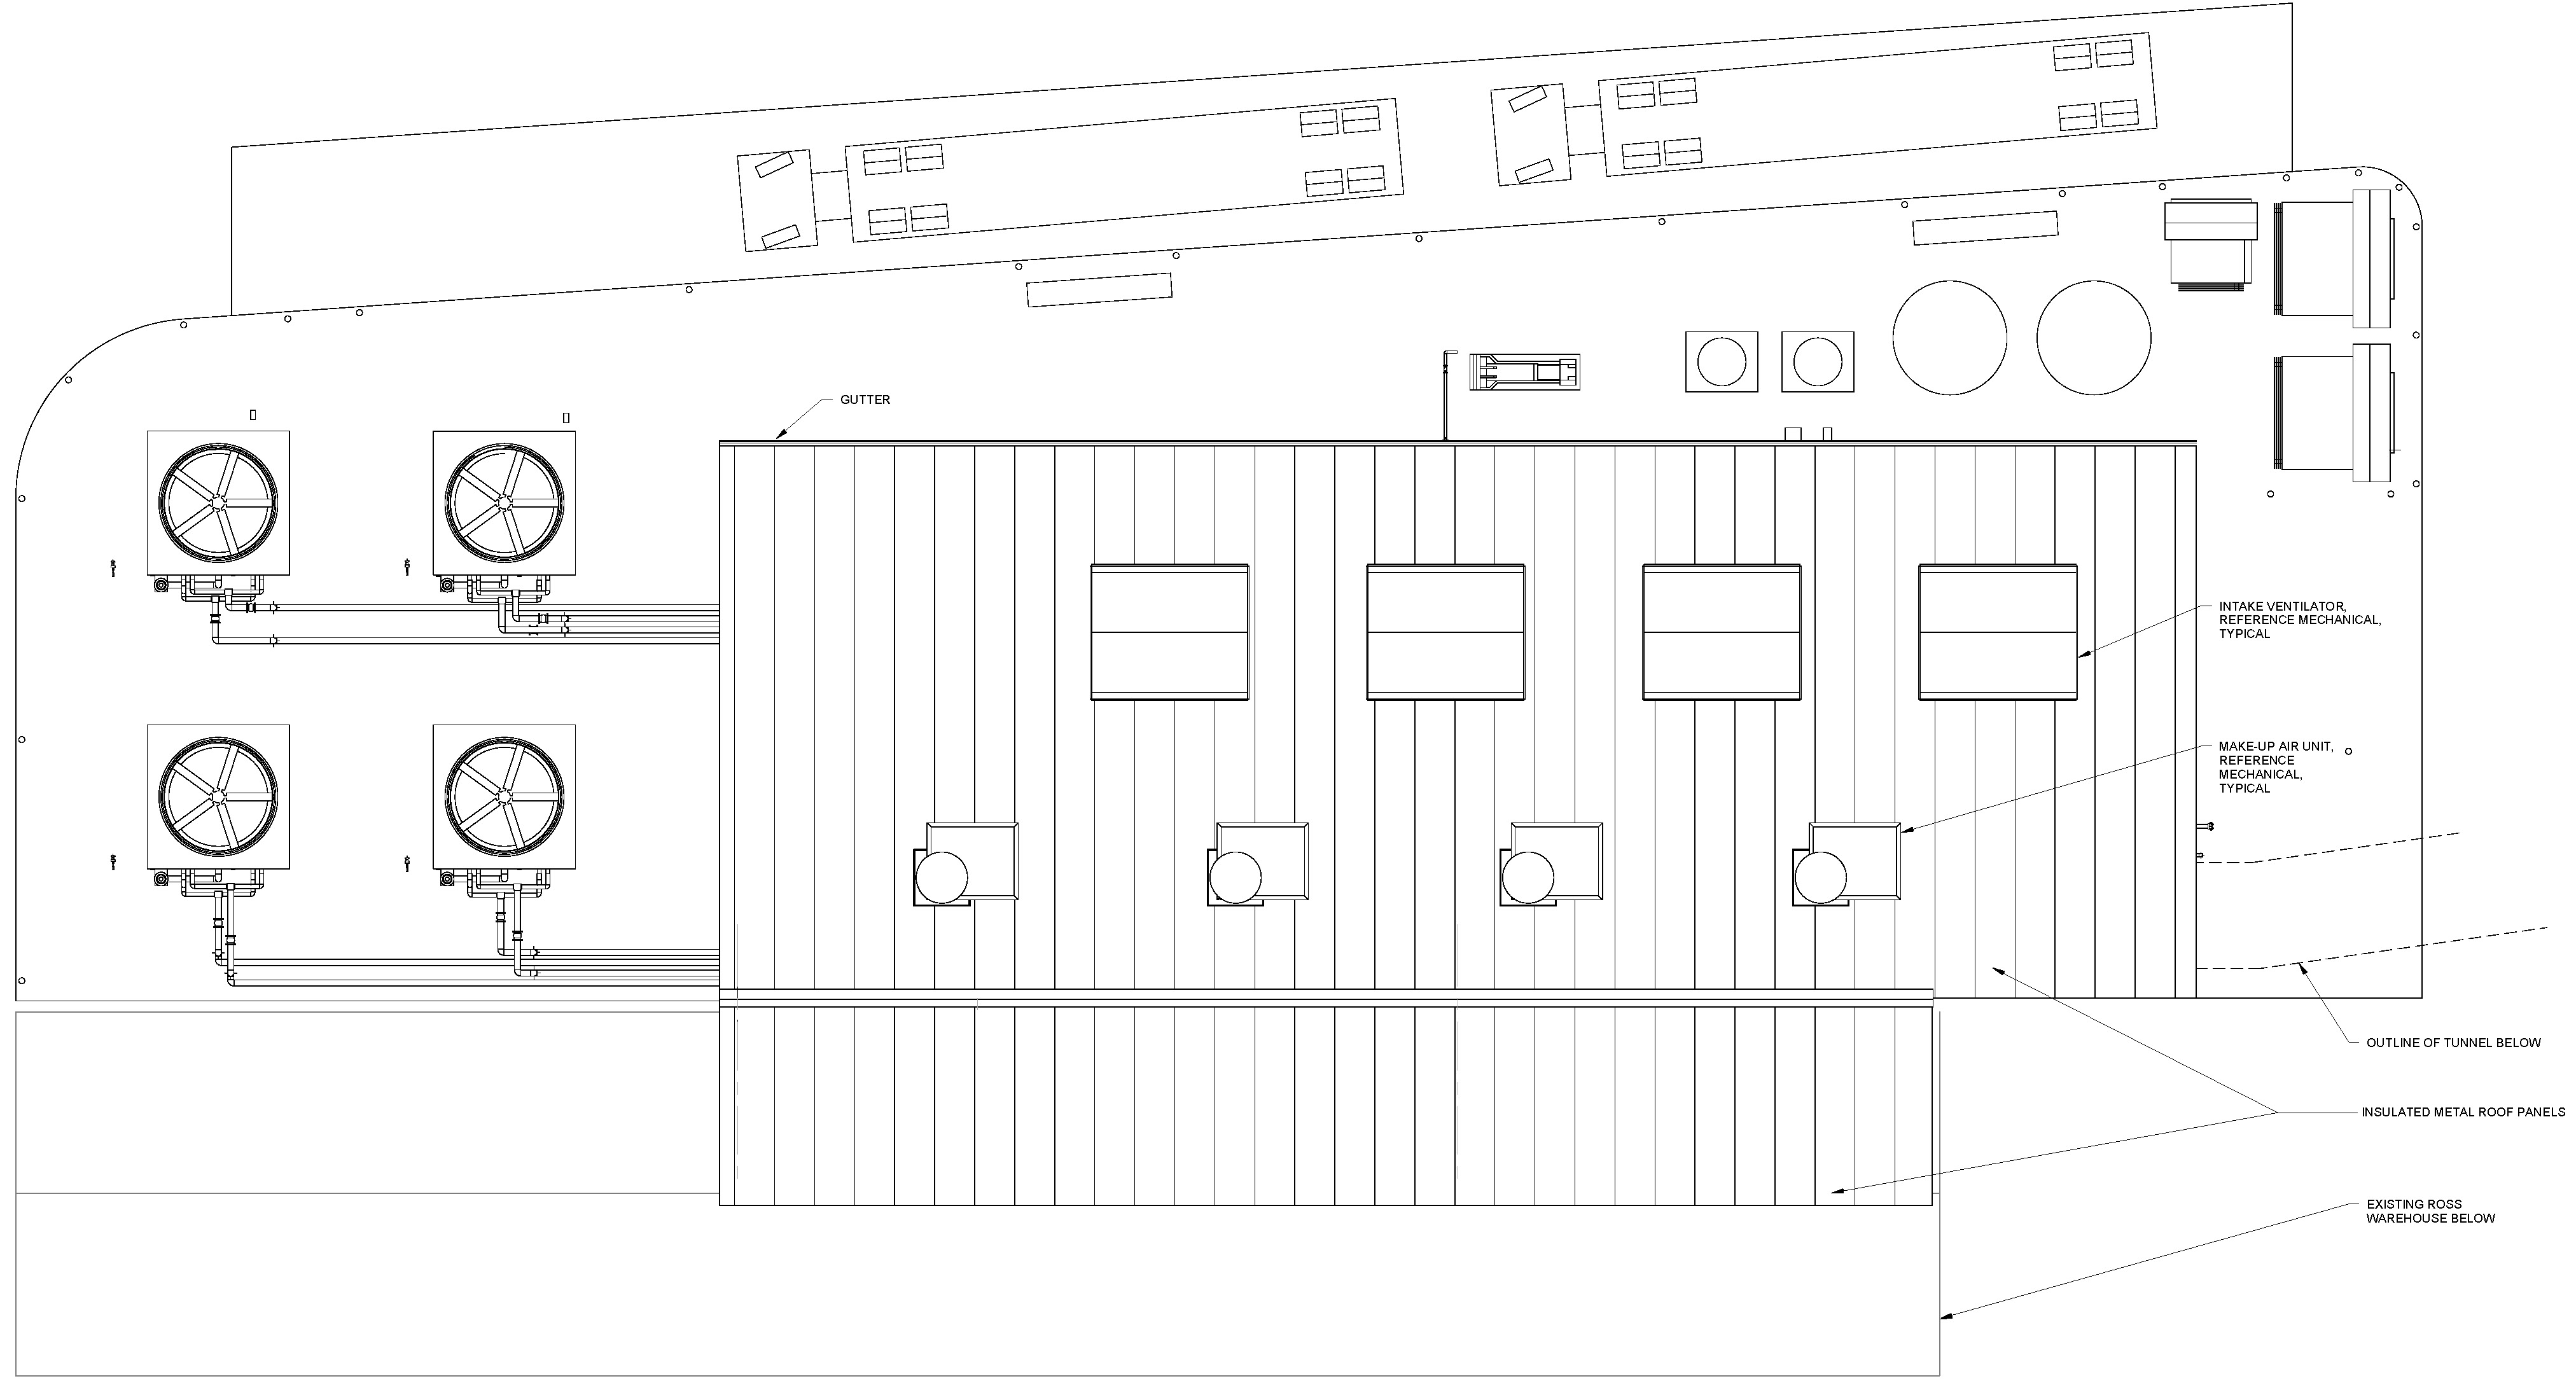
\includegraphics[width=\textwidth, angle=90]{compressor-bldg}
\end{cdrfigure}


%%%%%%%%%%%%%%%%%%%%%%%%%%%%%%%%%%
\subsection{Ross Dry Building}
\label{sec:fscf-surf-facil-surface-bldg-rossdry}

The Ross Dry building is in use by SURF to provide office and meeting space in addition to men's and women's locker room (or \textit{dry}) facilities and emergency response capabilities. As a scope option, the design includes a complete renovation of this building to upgrade these existing capabilities and to add space for an above-ground Control and Command Center.  (This control center itself is not a scope option; it could be placed in a different location.)  This design includes flexible space that can be tailored to %individual user's 
evolving needs as the project transitions from construction to operations. 

The exterior of the Ross Dry Building is shown in Figure~\ref{fig:ross-dry-ext}. The proposed renovations are shown in Figures~\ref{fig:cmd-control-center-main} and~\ref{fig:cmd-control-center-basement}.

\begin{cdrfigure}[Photo of Ross Dry exterior]{ross-dry-ext}{Photo of Ross Dry exterior (HDR) \fixme{Need orig; too fuzzy}}
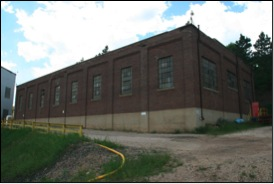
\includegraphics[width=0.8\textwidth]{ross-dry-ext}
\end{cdrfigure}

\begin{cdrfigure}[Location of new Command and Control Center (SURF), main floor.]{cmd-control-center-main}{Ross Dry Building renovation, main floor, showing the planned location for the control room (Command and Control Center). % could be located in any office space, but is planned for  the room at the bottom of this image.
}
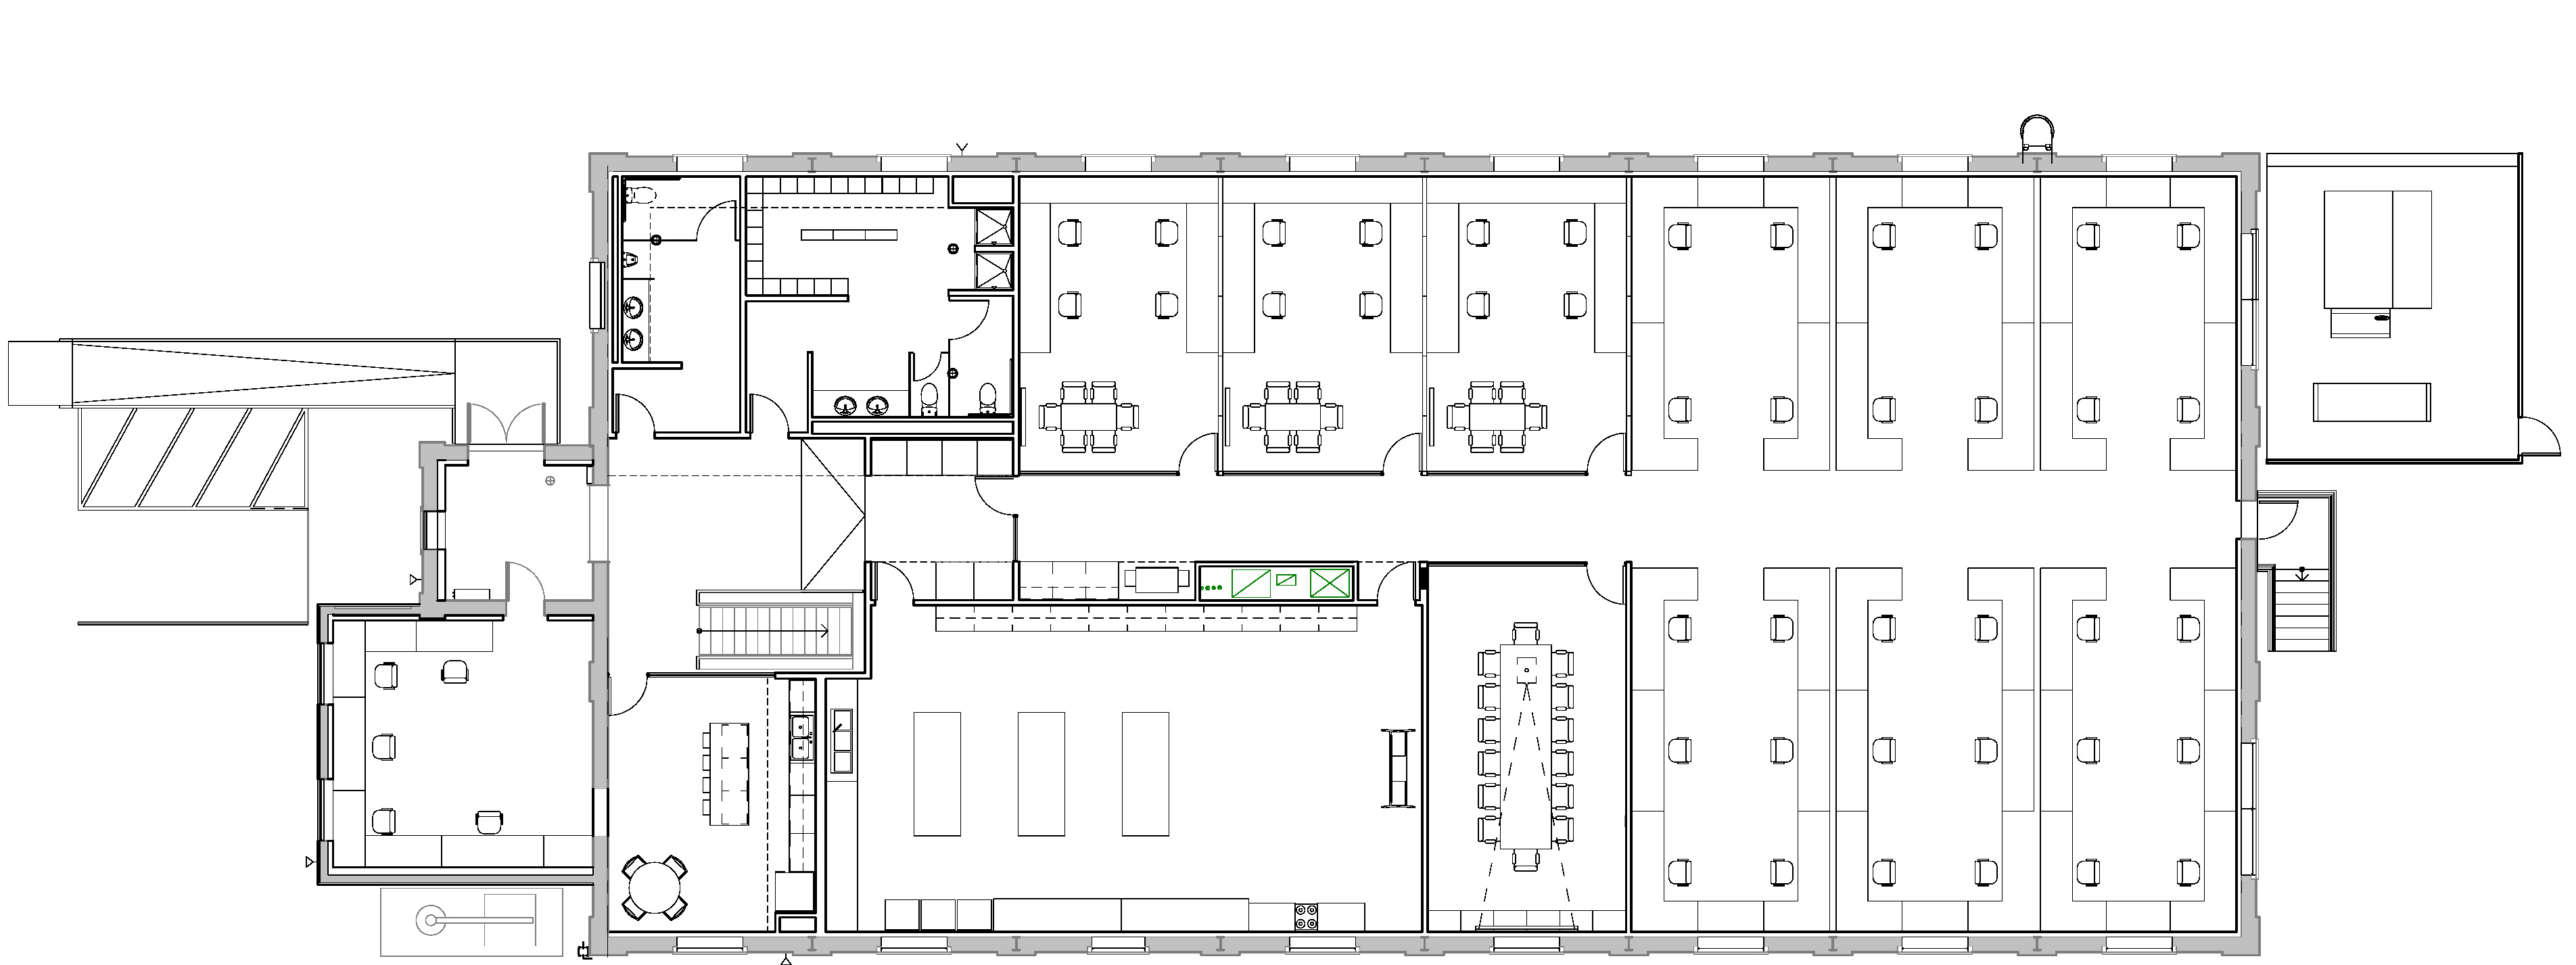
\includegraphics[width=1.25\textwidth, 
angle=90]{ross-dry-building-main-floor}
\end{cdrfigure}

\begin{cdrfigure}[Ross Dry Renovation, basement]{cmd-control-center-basement}{Ross Dry  Building renovation, basement.}
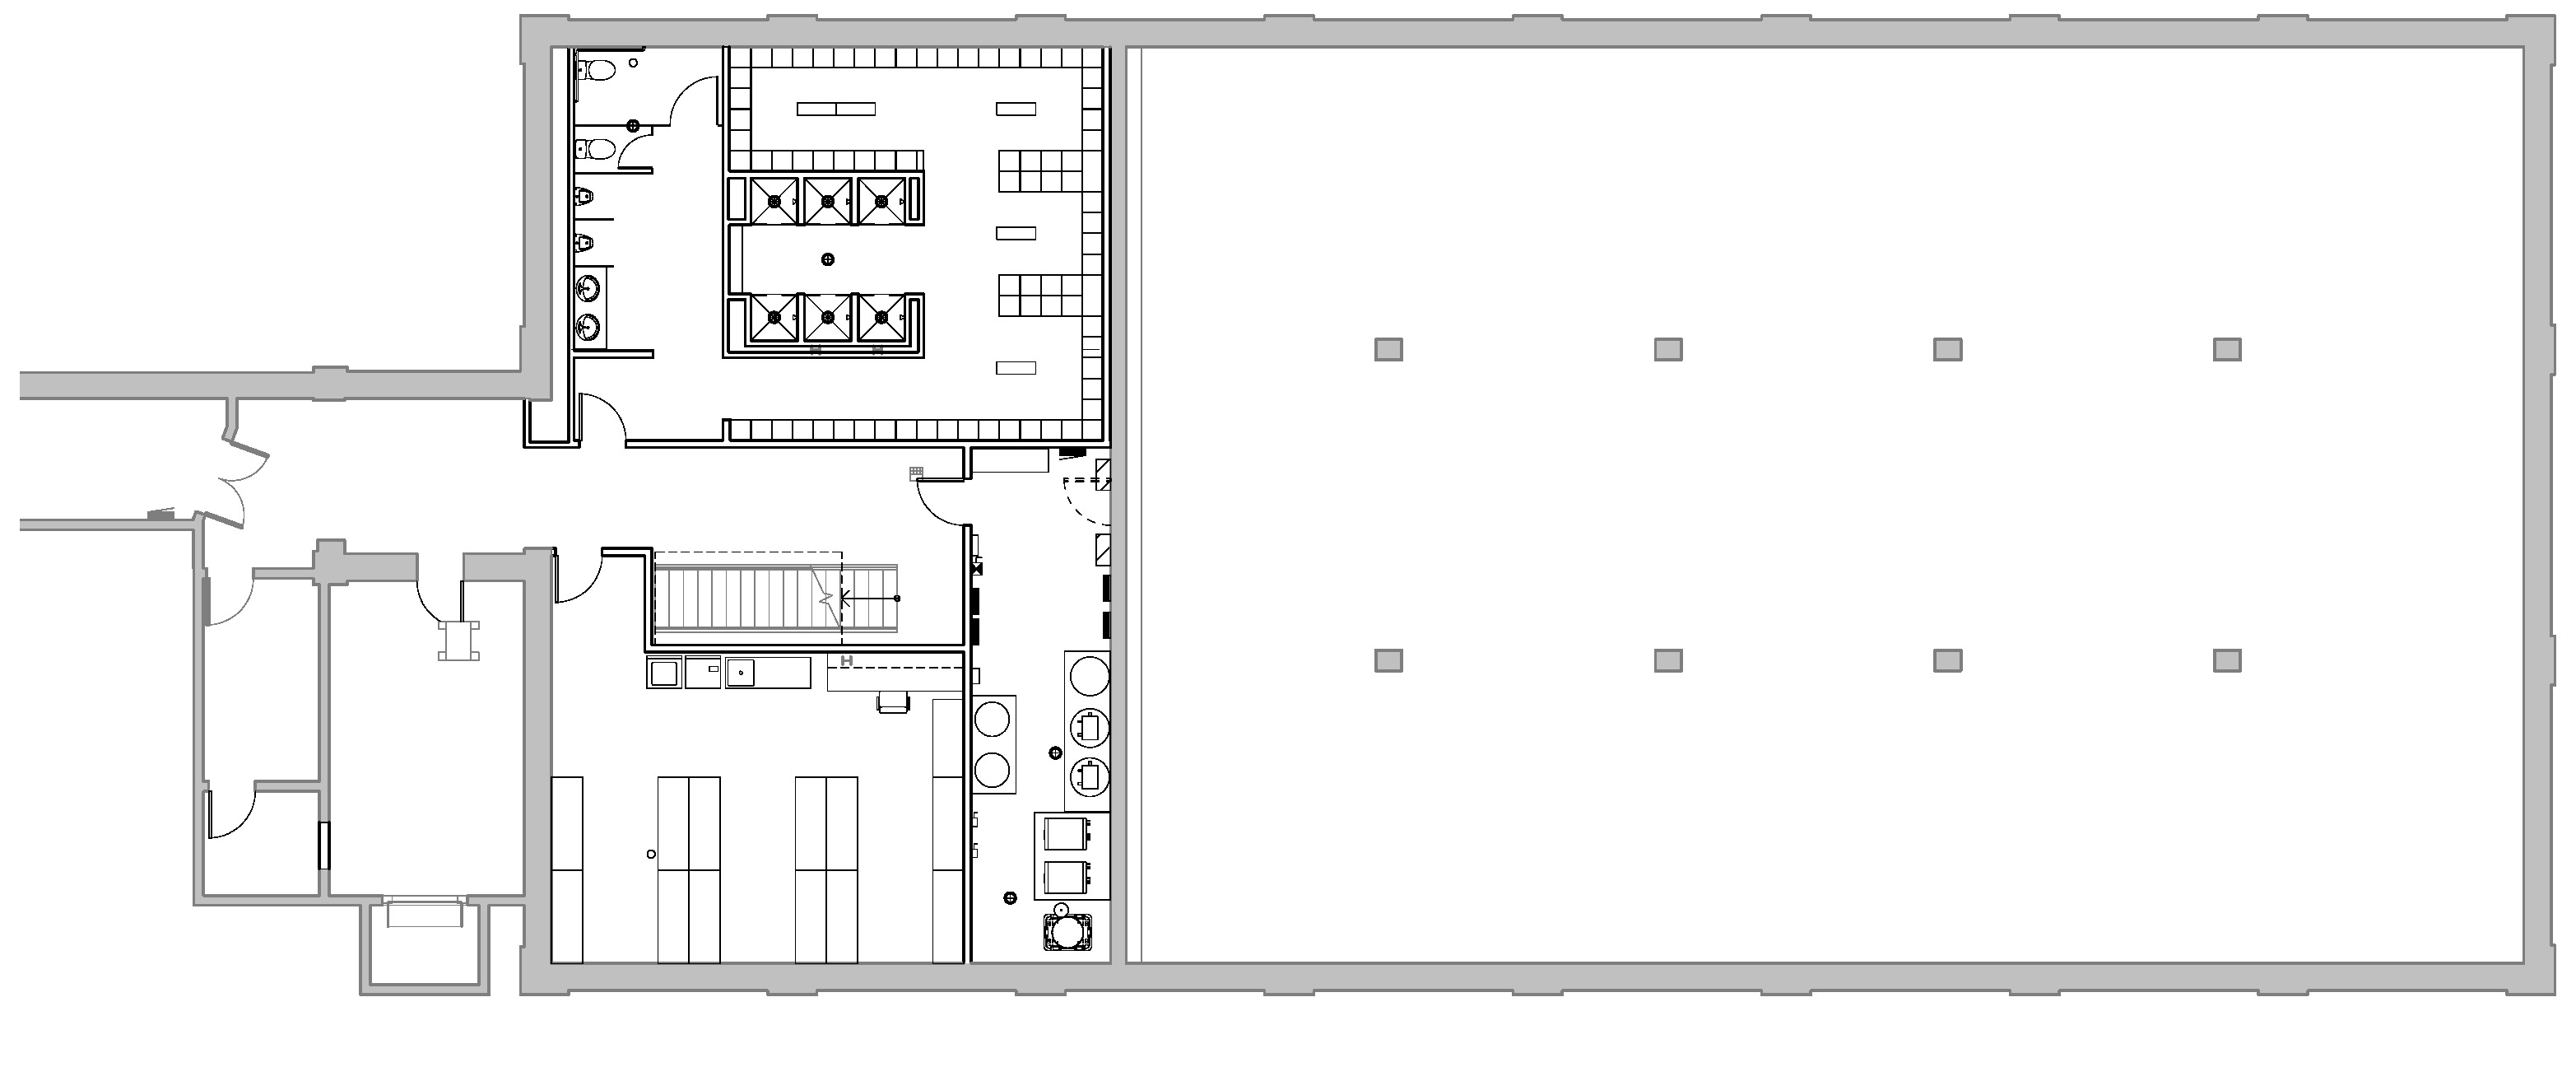
\includegraphics[width=1.25\textwidth, angle=90]{ross-dry-building-basement}
\end{cdrfigure}


%%%%%%%%%%%%%%%%%%%%%%%%%%%%%%%%%%
\subsection{Ross Headframe and Hoist Buildings}
\label{sec:fscf-surf-facil-surface-bldg-rosshead}

%The headframe and hoist buildings at the Ross Campus can be used by LBNF. %provide services for LBNF use. 
The Ross Headframe Building will be the main entry point for construction activities and for ongoing operations and maintenance functions. In addition, gas pipes from the LBNF Cryogenics Compressor Building will pass through this building on the way to the shaft.

Following shaft rehabilitation, the LBNF Project will include structural reinforcement of the Ross Headframe to meet current codes and standards.  The headframe will also be modified %somewhat 
to accommodate loads with dimensions longer than it can currently accommodate.  This project will occur concurrently with other site preparation activities planned to be performed outside of the CD-3a scope, as described in Chapter~\ref{ch:fscf-site-prep}.

\fixme{Not a word about the hoist building; change subsection title?}

%%%%%%%%%%%%%%%%%%%%%%%%%%%%%%%%%%
\subsection{Yates Headframe Building}
\label{sec:fscf-surf-facil-surface-bldg-yateshead}

The Yates Shaft, which terminates in the headframe building at the Yates Campus, will be used for delivery of personnel and materials underground during construction and operation of LBNF/DUNE.
The building and shaft will in fact be critical to LBNF during the installation of gas piping through the Ross Shaft, during which time the Ross Shaft will be restricted to that activity plus emergency egress.   The LBNF Project will therefore include structural reinforcement of the Yates Headframe to meet current codes and standards, to be completed prior to the installation of gas piping through the Ross shaft. % to ensure reliable operation during that time. 
Installation of a redundant fiber optic backbone through the Yates Shaft will provide a means to transfer DUNE data in the event of disruption of the fiber optic connection in the Ross Shaft, as well as for communications.

%The headframe at the Yates Campus provides services for LBNF use. One scope option is to provide a redundant fiber optic backbone through this shaft, and the shaft will be used for delivery of people and materials for construction and operation of LBNF.  One specific time frame where this shaft will be critical is during the installation of gas piping through the Ross shaft, during which time no other uses beyond emergency egress are possible.  Due to this demand, the LBNF project will include structural reinforcement of the Yates Headframe to meet current codes and standards.  This project will be completed prior to the installation of gas piping through the Ross shaft to ensure reliable operation during that time.


%%%%%%%%%%%%%%%%%%%%%%%%%%%%%%%%%%
\subsection{Ross Crusher Building}
\label{sec:fscf-surf-facil-surface-bldg-rosscrusher}

The existing Ross Crusher Building is a high-bay space that contains rock-crushing equipment used for construction operations. The exterior of the building will be repaired 
so that people can comfortably work inside. %to create a warm, usable shell. 
The upgrade of the existing crusher equipment is part of the waste rock handling work scope (see Section~\ref{sec:fscf-und-waste-rock}) and not part of the building rehabilitation. 

%%%%%%%%%%%%%%%%%%%%%%%%%%%%%%%%%%%%%%%%%%%%%%%%%%%%%%%%%%%%%%%%%%%
\section{New Surface Infrastructure}
\label{sec:fscf-surf-facil-surface-new}

Surface infrastructure includes items such as retaining walls and parking lots, as well as utilities to service both buildings and underground areas.  Existing infrastructure planned for use by LBNF requires both rehabilitation and upgrades to meet code and LBNF requirements. 
% (moved to first chapter)The experiment needs were documented in the requirements found in LBNF Requirements Document\cite{dune-sci-req} and combined with facility needs for the design detailed in the Arup 100\% Preliminary Design Report\cite{arup:fscf100pdr}.

No new roads or parking lots are required for LBNF at SURF. However, the Ross Complex site will require minor demolition of power lines and a fire hydrant that are no longer used in order to provide adequate accessibility for truck traffic to the new Cryogenics Compressor Building. An existing space will be designated for handicap parking adjacent to the Ross Dry Building. Additional road work is required for truck transportation of waste rock, as described in the waste rock handling section~\cite{sec:fscf-und-waste-rock}.




